\chapter{Forças intermoleculares e solventes}\label{ch:b1:intermolecular-forces-solvents}

Uma lagartixa sobe correndo por uma vidraça e fica pendurada por um
único dedo; sem cola, sem ventosa, apenas com a atração entre as
moléculas das almofadinhas de seus dedos e as do vidro. A água, uma
molécula mais leve que o dióxido de carbono, ferve a
\qty{100}{\celsius}, enquanto o dióxido de carbono é um gás à
temperatura ambiente. O óleo flutua sobre o vinagre e nunca se mistura
com ele; o sal de cozinha se dissolve na água e não na gasolina. Todos
esses fatos são decididos não pelas ligações dentro das moléculas, mas
pelas forças, muito mais fracas, entre elas. Este capítulo classifica
essas forças, mede seus efeitos sobre as temperaturas de ebulição e as
usa para escolher um solvente.

% ledger: bp:H2O (the hook's 100 degC)

\begin{recall}
O Livro 1 (ano 11) apresentou as forças de van der Waals e as \omterm{def:b1:intermolecular-forces-solvents:hbond}{ligações
de hidrogênio}, e explicou que os sólidos iônicos se dissolvem por
dissociação e \omterm{def:b1:intermolecular-forces-solvents:dissolution}{solvatação}. Os \omterm{def:b1:lewis-resonance-vsepr:dipole}{momentos dipolares} foram definidos na
\cref{def:b1:lewis-resonance-vsepr:dipole} e a \omterm{def:b1:periodicity:polarisability}{polarizabilidade} na
\cref{def:b1:periodicity:polarisability}. Da física, usamos a lei de
Coulomb: duas cargas $q_1$ e $q_2$ a uma distância
$r$ no vácuo se atraem ou se repelem com uma força de norma $|q_1q_2|/(4\pi
\varepsilon_0 r^2)$.
\end{recall}

\begin{omfigure}
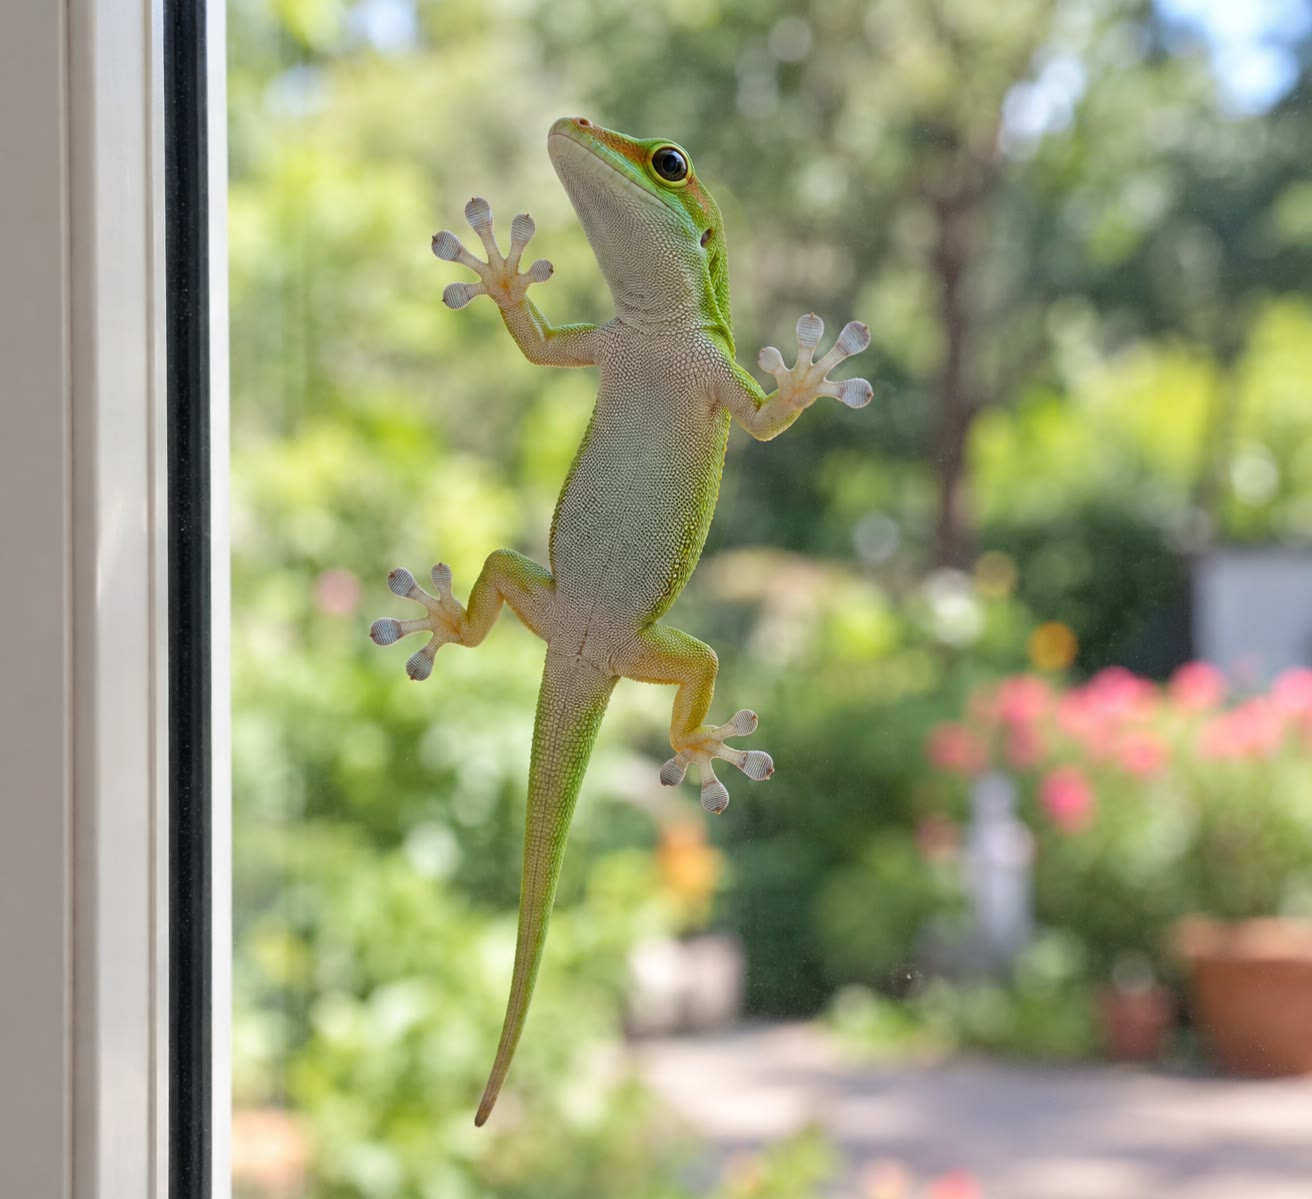
\includegraphics[width=0.52\linewidth]{images/book2/ai/b1-04-gecko.jpg}

{\small Uma lagartixa em uma vidraça. Os milhões de pelos finos das
almofadinhas de seus dedos chegam tão perto do vidro que a fraca atração
entre suas moléculas e as do vidro soma mais que o seu peso.}
\end{omfigure}

\section{Interações de van der Waals}

\begin{definition}[Interações de van der Waals]\label{def:b1:intermolecular-forces-solvents:vdw}
As \emph{interações de van der Waals}\index{interacao de van der Waals@interação de van der Waals}
são as atrações entre moléculas neutras que vêm da interação de seus
dipolos. Distinguem-se três tipos:
\begin{itemize}
  \item a \emph{interação de Keesom}\index{interacao de Keesom@interação de Keesom} (ou
        interação de orientação) entre dois dipolos permanentes, que
        tendem a se alinhar cabeça com cauda;
  \item a \emph{interação de Debye}\index{interacao de Debye@interação de Debye} (ou
        interação de indução) entre um dipolo permanente e o dipolo que
        ele induz em um vizinho polarizável;
  \item a \emph{interação de London}\index{interacao de London@interação de London} (ou
        interação de dispersão) entre os dipolos instantâneos que as
        flutuações das nuvens eletrônicas criam em quaisquer dois átomos
        ou moléculas, polares ou não, e que se induzem mutuamente.
\end{itemize}
\end{definition}

\begin{omfigure}
\begin{tikzpicture}[font=\small, >={Stealth},
    mol/.style={draw=black!60, fill=#1, ellipse, minimum width=1.5cm, minimum height=0.8cm}]
  % Keesom
  \node[mol=omDef!20] (a) at (0,0) {}; \node[mol=omDef!20] (b) at (1.7,0) {};
  \node at (-0.45,0) {$\delta^-$}; \node at (0.45,0) {$\delta^+$};
  \node at (1.25,0) {$\delta^-$}; \node at (2.15,0) {$\delta^+$};
  \node[below, align=center] at (0.85,-0.65) {Keesom:\\dois dipolos permanentes};
  % Debye
  \begin{scope}[xshift=4.6cm]
    \node[mol=omDef!20] at (0,0) {}; \node[mol=black!5, dashed] at (1.7,0) {};
    \node at (-0.45,0) {$\delta^-$}; \node at (0.45,0) {$\delta^+$};
    \node[omProp] at (1.25,0) {$\delta^-$}; \node[omProp] at (2.15,0) {$\delta^+$};
    \node[below, align=center] at (0.85,-0.65) {Debye:\\permanente e induzido};
  \end{scope}
  % London
  \begin{scope}[xshift=9.2cm]
    \node[mol=black!5, dashed] at (0,0) {}; \node[mol=black!5, dashed] at (1.7,0) {};
    \node[omProp] at (-0.45,0) {$\delta^-$}; \node[omProp] at (0.45,0) {$\delta^+$};
    \node[omProp] at (1.25,0) {$\delta^-$}; \node[omProp] at (2.15,0) {$\delta^+$};
    \node[below, align=center] at (0.85,-0.65) {London:\\dois dipolos instantâneos};
  \end{scope}
\end{tikzpicture}

{\small As três \omterm{def:b1:intermolecular-forces-solvents:vdw}{interações de van der Waals}. As cargas parciais em preto
são permanentes (\omterm{def:b1:lewis-resonance-vsepr:dipole}{moléculas polares}); as em laranja são induzidas ou
instantâneas. Em cada caso, as cargas frente a frente são opostas, de
modo que as moléculas se atraem.}
\end{omfigure}

\begin{proposition}[Intensidade e alcance]\label{prop:b1:intermolecular-forces-solvents:distance-law}
Para duas moléculas a uma distância $r$, cada uma das três energias de
van der Waals varia como $-1/r^6$: a atração só se faz sentir entre
vizinhos. Suas energias são da ordem de alguns quilojoules por mol,
cerca de cem vezes menos que uma \omterm{def:b1:lewis-resonance-vsepr:lewis}{ligação covalente}. O termo de London
cresce com as \omterm{def:b1:periodicity:polarisability}{polarizabilidades} dos dois parceiros; ele está presente
entre todas as moléculas e costuma ser o maior dos três, exceto para
moléculas pequenas e muito polares.
\end{proposition}
\admitted

\begin{example}[Gases nobres e halogênios]\label{ex:b1:intermolecular-forces-solvents:noble}
Os átomos de um gás nobre se atraem apenas por forças de London, que
crescem com o número de elétrons: o hélio ferve a
\qty{-268.9}{\celsius}, o neônio a \qty{-246.1}{\celsius}, o argônio a
\qty{-185.9}{\celsius}, o criptônio a \qty{-153.4}{\celsius}, o xenônio a
\qty{-108.1}{\celsius}. Da mesma forma, à temperatura ambiente, o
diflúor e o dicloro são gases, o dibromo é um líquido (que ferve a
\qty{58.8}{\celsius}) e o di-iodo é um sólido.
% ledger: bp:He, bp:Ne, bp:Ar, bp:Kr, bp:Xe, bp:F2, bp:Cl2, bp:Br2, bp:I2
\end{example}

\begin{omfigure}
\begin{tikzpicture}
\begin{axis}[
  width=0.62\linewidth, height=5.4cm,
  xmin=0.5, xmax=10.5, ymin=-180, ymax=200,
  axis x line=bottom, axis y line=left,
  xlabel={número de átomos de carbono $n$}, ylabel={temperatura de ebulição (\unit{\celsius})},
  xtick={1,2,3,4,5,6,7,8,9,10}, ytick={-150,-100,-50,0,50,100,150},
  tick label style={font=\small}, label style={font=\small}]
\addplot[omDef, thick, mark=*, mark size=1.5pt] table[x=n, y=bp_C] {figdata/out/bachelor-1-hydride-boiling-points-alkanes.dat};
\end{axis}
\end{tikzpicture}

{\small Temperaturas de ebulição dos alcanos lineares \ce{C_nH_{2n+2}},
do metano ao decano. Cada \ce{CH2} acrescentado adiciona elétrons e
superfície de contato, portanto atração de London; o incremento diminui
lentamente, de cerca de \qty{75}{\celsius} no início a \qty{25}{\celsius}
no decano.}
\end{omfigure}

\section{A ligação de hidrogênio}

\begin{definition}[Ligação de hidrogênio]\label{def:b1:intermolecular-forces-solvents:hbond}
Uma \emph{ligação de hidrogênio}\index{ligacao de hidrogenio@ligação de hidrogênio} é uma atração
$\ce{X-H}\cdots\ce{Y}$ entre um átomo de hidrogênio ligado a um átomo X
pequeno e muito eletronegativo (\ce{N}, \ce{O} ou \ce{F}) e um \omterm{def:b1:lewis-resonance-vsepr:lewis}{par não
ligante} de outro átomo eletronegativo Y. A molécula que leva \ce{X-H} é o
doador da ligação de hidrogênio; a que leva Y, o aceptor. Sua energia, de
10 a \qty{40}{kJ/mol}, fica entre a das \omterm{def:b1:intermolecular-forces-solvents:vdw}{interações de van der Waals} e a
das \omterm{def:b1:lewis-resonance-vsepr:lewis}{ligações covalentes}; os três átomos \ce{X}, \ce{H}, \ce{Y} estão
quase alinhados.
\end{definition}

\begin{remark}[Por que N, O e F]\label{rem:b1:intermolecular-forces-solvents:why}
Um X fortemente eletronegativo deixa o hidrogênio com uma grande carga
parcial positiva; o hidrogênio, que não tem elétrons internos, é
minúsculo, de modo que o \omterm{def:b1:lewis-resonance-vsepr:lewis}{par não ligante} de Y pode chegar muito perto
dele. As duas condições são necessárias: as ligações \ce{C-H} não são
polares o suficiente, e as ligações \ce{S-H} ou \ce{Cl-H} envolvem
átomos grandes demais e pouco eletronegativos demais para formar
\omterm{def:b1:intermolecular-forces-solvents:hbond}{ligações de hidrogênio} fortes.
\end{remark}

\begin{omfigure}
\begin{tikzpicture}[font=\small]
  % water network
  \foreach \n/\x/\y/\a in {1/0/0/0, 2/2.2/0.9/200, 3/0.2/-2.0/60, 4/-2.1/0.6/-30} {
    \begin{scope}[shift={(\x,\y)}, rotate=\a]
      \node[aO] (o\n) at (0,0) {};
      \node[aH] (h\n a) at (0.78,0.3) {};
      \node[aH] (h\n b) at (-0.2,-0.82) {};
      \begin{scope}[on background layer]
        \draw[bond] (o\n.center) -- (h\n a.center); \draw[bond] (o\n.center) -- (h\n b.center);
      \end{scope}
    \end{scope}
  }
  \draw[omThm, thick, densely dotted] (h1a) -- (o2);
  \draw[omThm, thick, densely dotted] (h1b) -- (o3);
  \draw[omThm, thick, densely dotted] (h4a) -- (o1);
  \node[below] at (0,-2.9) {água: cada molécula pode doar duas e aceitar duas};
  % carboxylic acid dimer
  \begin{scope}[xshift=5.6cm, yshift=-0.6cm]
    \node (r1) at (-0.9,0) {R}; \node (c1) at (0,0) {C};
    \node (o1) at (0.6,0.85) {O}; \node (o2) at (0.6,-0.85) {O}; \node (h2) at (1.45,-0.85) {H};
    \node (c2) at (3.3,0) {C}; \node (r2) at (4.2,0) {R};
    \node (o3) at (2.7,0.85) {O}; \node (o4) at (2.7,-0.85) {O}; \node (h3) at (1.85,0.85) {H};
    \draw (r1) -- (c1) -- (o2) -- (h2) (c2) -- (r2) (c2) -- (o3) -- (h3);
    \draw[double, double distance=1.6pt] (c1) -- (o1); \draw[double, double distance=1.6pt] (c2) -- (o4);
    \draw[omThm, thick, densely dotted] (h2) -- (o4) (h3) -- (o1);
    \node[below] at (1.65,-2.3) {um dímero de ácido carboxílico};
  \end{scope}
\end{tikzpicture}

{\small \omterm{def:b1:intermolecular-forces-solvents:hbond}{Ligações de hidrogênio} (pontilhado vermelho). Na água líquida,
cada molécula participa de até quatro delas; os ácidos carboxílicos se
emparelham em dímeros cíclicos mantidos por duas \omterm{def:b1:intermolecular-forces-solvents:hbond}{ligações de hidrogênio}.}
\end{omfigure}

\begin{proposition}[As ligações de hidrogênio elevam as temperaturas de ebulição]\label{prop:b1:intermolecular-forces-solvents:hbond-bp}
Entre os hidretos dos \omterm{def:b1:periodicity:table}{grupos} 15, 16 e 17, a temperatura de ebulição
aumenta do \omterm{def:b1:periodicity:table}{período} 3 ao \omterm{def:b1:periodicity:table}{período} 5, acompanhando a \omterm{def:b1:intermolecular-forces-solvents:vdw}{interação de London};
os hidretos do \omterm{def:b1:periodicity:table}{período} 2, \ce{NH3}, \ce{H2O} e \ce{HF}, que formam
\omterm{def:b1:intermolecular-forces-solvents:hbond}{ligações de hidrogênio}, fervem muito acima da extrapolação dessa
tendência. Os hidretos do \omterm{def:b1:periodicity:table}{grupo} 14 (\ce{CH4}, \ce{SiH4}, \ce{GeH4}) não
formam \omterm{def:b1:intermolecular-forces-solvents:hbond}{ligações de hidrogênio} e seguem a tendência.
\end{proposition}

\begin{omfigure}
\begin{tikzpicture}
\begin{axis}[
  width=0.82\linewidth, height=6.6cm,
  xmin=1.5, xmax=5.6, ymin=-180, ymax=120,
  axis x line=bottom, axis y line=left,
  xlabel={período}, ylabel={temperatura de ebulição (\unit{\celsius})},
  xtick={2,3,4,5}, ytick={-150,-100,-50,0,50,100},
  tick label style={font=\small}, label style={font=\small},
  clip=false]
\addplot[black!60, thick, mark=square*, mark size=1.6pt] table[x=period, y=bp_C] {figdata/out/bachelor-1-hydride-boiling-points-g14.dat};
\addplot[omDef, thick, mark=*, mark size=1.6pt] table[x=period, y=bp_C] {figdata/out/bachelor-1-hydride-boiling-points-g15.dat};
\addplot[omThm, thick, mark=*, mark size=1.6pt] table[x=period, y=bp_C] {figdata/out/bachelor-1-hydride-boiling-points-g16.dat};
\addplot[omMeth, thick, mark=triangle*, mark size=2pt] table[x=period, y=bp_C] {figdata/out/bachelor-1-hydride-boiling-points-g17.dat};
\addplot[omThm, dashed] coordinates {(2,-79.3) (3,-60.3)};
\node[font=\small, anchor=west] at (axis cs:2.05,100) {\ce{H2O}};
\node[font=\small, anchor=west] at (axis cs:2.05,19.6) {\ce{HF}};
\node[font=\small, anchor=west] at (axis cs:2.05,-30) {\ce{NH3}};
\node[font=\small, anchor=east] at (axis cs:1.96,-162) {\ce{CH4}};
\node[font=\small, anchor=west] at (axis cs:4.05,-41.3) {\ce{H2Se}};
\node[font=\small, anchor=west] at (axis cs:5.05,-18.4) {\ce{SbH3}};
\node[font=\small, anchor=west] at (axis cs:5.05,-35.1) {\ce{HI}};
\node[font=\small, anchor=west] at (axis cs:4.05,-88.1) {\ce{GeH4}};
\node[font=\small, omThm, anchor=north west] at (axis cs:2.05,-85) {extrapolado};
\end{axis}
\end{tikzpicture}

{\small Temperaturas de ebulição dos hidretos dos \omterm{def:b1:periodicity:table}{grupos} 14 (quadrados
cinza), 15 (azul), 16 (vermelho) e 17 (verde). A água ferveria perto de
\qty{-79}{\celsius} se seguisse seus análogos mais pesados (tracejado);
suas \omterm{def:b1:intermolecular-forces-solvents:hbond}{ligações de hidrogênio} a elevam em cerca de \qty{180}{\celsius}.}
% ledger: bp:CH4, bp:SiH4, bp:GeH4, bp:NH3, bp:PH3, bp:AsH3, bp:SbH3,
% bp:H2O, bp:H2S, bp:H2Se, bp:HF, bp:HCl, bp:HBr, bp:HI
\end{omfigure}

\begin{example}[O etanol e seu isômero]\label{ex:b1:intermolecular-forces-solvents:isomers}
O etanol, \ce{CH3CH2OH}, e o metoximetano, \ce{CH3OCH3}, têm a mesma
fórmula \ce{C2H6O} e quase as mesmas \omterm{def:b1:intermolecular-forces-solvents:vdw}{interações de London}. O etanol,
cujo grupo \ce{O-H} é ao mesmo tempo doador e aceptor, ferve a
\qty{78.4}{\celsius}; o metoximetano, que só pode aceitar, ferve a
\qty{-25.0}{\celsius}.
% ledger: bp:C2H5OH, bp:CH3OCH3
\end{example}

\section{Solventes}

\begin{definition}[Permissividade relativa]\label{def:b1:intermolecular-forces-solvents:permittivity}
Em um meio, a força de Coulomb entre duas cargas é dividida por um número
$\varepsilon_r \ge 1$, a \emph{permissividade relativa}\index{permissividade relativa}
(ou constante dielétrica) do meio:
\[
  F = \frac{|q_1 q_2|}{4\pi\varepsilon_0\varepsilon_r r^2} .
\]
Ela é grande para líquidos de \omterm{def:b1:lewis-resonance-vsepr:dipole}{moléculas polares}, que se orientam em
torno das cargas e as blindam: \num{78.4} para a água a \qty{25}{\celsius},
\num{1.89} para o hexano a \qty{20}{\celsius}.
% ledger: epsr:H2O, epsr:C6H14
\end{definition}

\begin{definition}[Solventes polares, próticos e apróticos]\label{def:b1:intermolecular-forces-solvents:solvent-classes}
Um \emph{solvente polar}\index{solvente polar} é formado por moléculas
com grande \omterm{def:b1:lewis-resonance-vsepr:dipole}{momento dipolar} e tem grande \omterm{def:b1:intermolecular-forces-solvents:permittivity}{permissividade relativa} (acima
de cerca de 15); um solvente apolar tem permissividade pequena. Um
\emph{solvente prótico}\index{solvente protico@solvente prótico} tem moléculas que levam átomos de
hidrogênio capazes de formar \omterm{def:b1:intermolecular-forces-solvents:hbond}{ligações de hidrogênio} (\ce{O-H} ou
\ce{N-H}); um \emph{solvente aprótico}\index{solvente aprotico@solvente aprótico} não tem nenhum.
\end{definition}

\begin{center}
\small
\begin{tabular}{lccll}
\hline
solvente & $\varepsilon_r$ & $\mu$ (D) & polaridade & proticidade \\
\hline
água & 78.4 & 1.86 & polar & prótico \\
metanol & 32.6 & 1.67 & polar & prótico \\
etanol & 24.3 & 1.52 & polar & prótico \\
acetonitrila, \ce{CH3CN} & 37.5 & 3.92 & polar & aprótico \\
propanona (acetona) & 20.7 & 2.88 & polar & aprótico \\
diclorometano & 9.08 & 1.62 & pouco polar & aprótico \\
etanoato de etila & 6.02 & 1.78 & pouco polar & aprótico \\
etoxietano & 4.34 & 1.15 & pouco polar & aprótico \\
benzeno & 2.28 & 0 & apolar & aprótico \\
hexano & 1.89 & 0 & apolar & aprótico \\
\hline
\end{tabular}
\end{center}
% ledger: epsr:H2O, epsr:CH3OH, epsr:C2H5OH, epsr:CH3CN, epsr:CH3COCH3,
% epsr:CH2Cl2, epsr:EtOAc, epsr:Et2O, epsr:C6H6, epsr:C6H14, dip:H2O,
% dip:CH3OH, dip:C2H5OH, dip:CH3CN, dip:CH3COCH3, dip:CH2Cl2, dip:EtOAc,
% dip:Et2O, dip:C6H6 (relative permittivities at 20 or 25 degC; dipole
% moments of the gas-phase molecules; hexane has no dipole by symmetry)

\begin{definition}[Solvatação, poder ionizante e poder dissociante]\label{def:b1:intermolecular-forces-solvents:dissolution}
A \emph{solvatação}\index{solvatacao@solvatação} de uma partícula de soluto é o seu
envolvimento por moléculas de solvente orientadas e ligadas a ela por
forças intermoleculares (hidratação, na água). O \emph{poder
ionizante}\index{poder ionizante} de um solvente é sua capacidade de
transformar uma \omterm{def:b1:lewis-resonance-vsepr:lewis}{ligação covalente} polar do soluto em um par de íons,
propriedade dos \omterm{def:b1:intermolecular-forces-solvents:solvent-classes}{solventes polares} de grande \omterm{def:b1:lewis-resonance-vsepr:dipole}{momento dipolar}; seu
\emph{poder dissociante}\index{poder dissociante} é sua capacidade de
separar os íons de um par, medida por sua \omterm{def:b1:intermolecular-forces-solvents:permittivity}{permissividade relativa}.
\end{definition}

\begin{proposition}[A dissolução em três etapas]\label{prop:b1:intermolecular-forces-solvents:steps}
A dissolução de um eletrólito em um solvente pode ser descrita em três
etapas: ionização (para um soluto molecular como \ce{HCl}), dissociação
dos pares de íons e \omterm{def:b1:intermolecular-forces-solvents:dissolution}{solvatação} dos íons separados. Um solvente dissolve
bem um soluto iônico ou muito polar quando é polar (ionizante), de alta
permissividade (dissociante) e capaz de solvatar os dois íons --- os
cátions por seus \omterm{def:b1:lewis-resonance-vsepr:lewis}{pares não ligantes}, os ânions por \omterm{def:b1:intermolecular-forces-solvents:hbond}{ligações de
hidrogênio}, se for prótico. A água faz as três coisas.
\end{proposition}

\begin{example}[O cloreto de hidrogênio na água e no hexano]\label{ex:b1:intermolecular-forces-solvents:hcl}
Na água, \ce{HCl} é ionizado e dissociado completamente:
\ce{HCl(g) + H2O(l) -> H3O+(aq) + Cl-(aq)}; a solução conduz. No
hexano, apolar e de baixa permissividade, ele se dissolve na forma de
moléculas de \ce{HCl} e a solução não conduz.
\end{example}

\begin{omfigure}
\begin{tikzpicture}[font=\small]
  \node[aNa] (na) at (0,0) {};
  \node[font=\scriptsize, white] at (na) {\ce{Na+}};
  \foreach \a in {0,60,...,300} {
    \begin{scope}[shift={(\a:1.25)}, rotate=\a]
      \node[aO] (o) at (0,0) {};
      \node[aH] (ha) at (0.55,0.5) {}; \node[aH] (hb) at (0.55,-0.5) {};
      \begin{scope}[on background layer]
        \draw[bond] (o.center) -- (ha.center); \draw[bond] (o.center) -- (hb.center);
      \end{scope}
    \end{scope}
  }
  \node[below] at (0,-2.4) {\shortstack{cátion: pares não ligantes\\do oxigênio para dentro}};
  \begin{scope}[xshift=6.2cm]
    \node[aCl] (cl) at (0,0) {};
    \node[font=\scriptsize, white] at (cl) {\ce{Cl-}};
    \foreach \a in {0,60,...,300} {
      \begin{scope}[shift={(\a:1.55)}, rotate=\a]
        \node[aH] (h1) at (-0.62,0) {};
        \node[aO] (o) at (0,0) {};
        \node[aH] (h2) at (0.25,0.72) {};
        \begin{scope}[on background layer]
          \draw[bond] (o.center) -- (h1.center); \draw[bond] (o.center) -- (h2.center);
        \end{scope}
      \end{scope}
    }
    \node[below] at (0,-2.4) {\shortstack{ânion: ligações de\\hidrogênio para dentro}};
  \end{scope}
\end{tikzpicture}

{\small Hidratação dos dois íons do cloreto de sódio (apenas a primeira
camada, desenhada no plano). A água volta sua extremidade negativa, o
oxigênio, para o cátion, e um hidrogênio para o ânion.}
\end{omfigure}

\section{Solubilidade, miscibilidade e anfifílicos}

\begin{proposition}[Semelhante dissolve semelhante]\label{prop:b1:intermolecular-forces-solvents:like}
Um soluto se dissolve bem em um solvente quando as interações entre as
moléculas de soluto e de solvente são comparáveis às que elas perdem:
solutos polares ou formadores de íons em \omterm{def:b1:intermolecular-forces-solvents:solvent-classes}{solventes polares}, solutos
apolares em solventes apolares, solutos que formam \omterm{def:b1:intermolecular-forces-solvents:hbond}{ligações de
hidrogênio} em \omterm{def:b1:intermolecular-forces-solvents:solvent-classes}{solventes próticos}.
\end{proposition}

\begin{proof}[Raciocínio]
Dissolver rompe interações soluto--soluto e solvente--solvente e forma
interações soluto--solvente. Se o soluto é apolar e o solvente é a água,
as moléculas de água perdem \omterm{def:b1:intermolecular-forces-solvents:hbond}{ligações de hidrogênio} para lhe abrir espaço
e só ganham em troca fracas \omterm{def:b1:intermolecular-forces-solvents:vdw}{interações de London}: a dissolução é
desfavorável. Se ambos são apolares, as \omterm{def:b1:intermolecular-forces-solvents:vdw}{interações de London} perdidas e
ganhas são comparáveis, e a mistura é favorecida pela desordem que cria.
\end{proof}

\begin{definition}[Líquidos miscíveis]\label{def:b1:intermolecular-forces-solvents:miscibility}
Dois líquidos são \emph{miscíveis}\index{miscivel@miscível} quando se misturam em
quaisquer proporções formando uma única fase líquida; caso contrário,
formam duas camadas, com a menos densa por cima.
\end{definition}

\begin{example}[Água com etanol, água com hexano]\label{ex:b1:intermolecular-forces-solvents:miscible}
O etanol é \omterm{def:b1:intermolecular-forces-solvents:miscibility}{miscível} com a água: ambos são próticos e polares, e o etanol
forma \omterm{def:b1:intermolecular-forces-solvents:hbond}{ligações de hidrogênio} com a água tanto quanto consigo mesmo. O
hexano e a água são imiscíveis. O di-iodo, um sólido molecular, é pouco
solúvel em água, mas se dissolve facilmente no hexano ou no
diclorometano: agitado com um desses solventes, o iodo aquoso passa para
a fase orgânica, o princípio da extração líquido--líquido
(\cref{ch:b1:lab-techniques-1}).
\end{example}

\begin{omfigure}
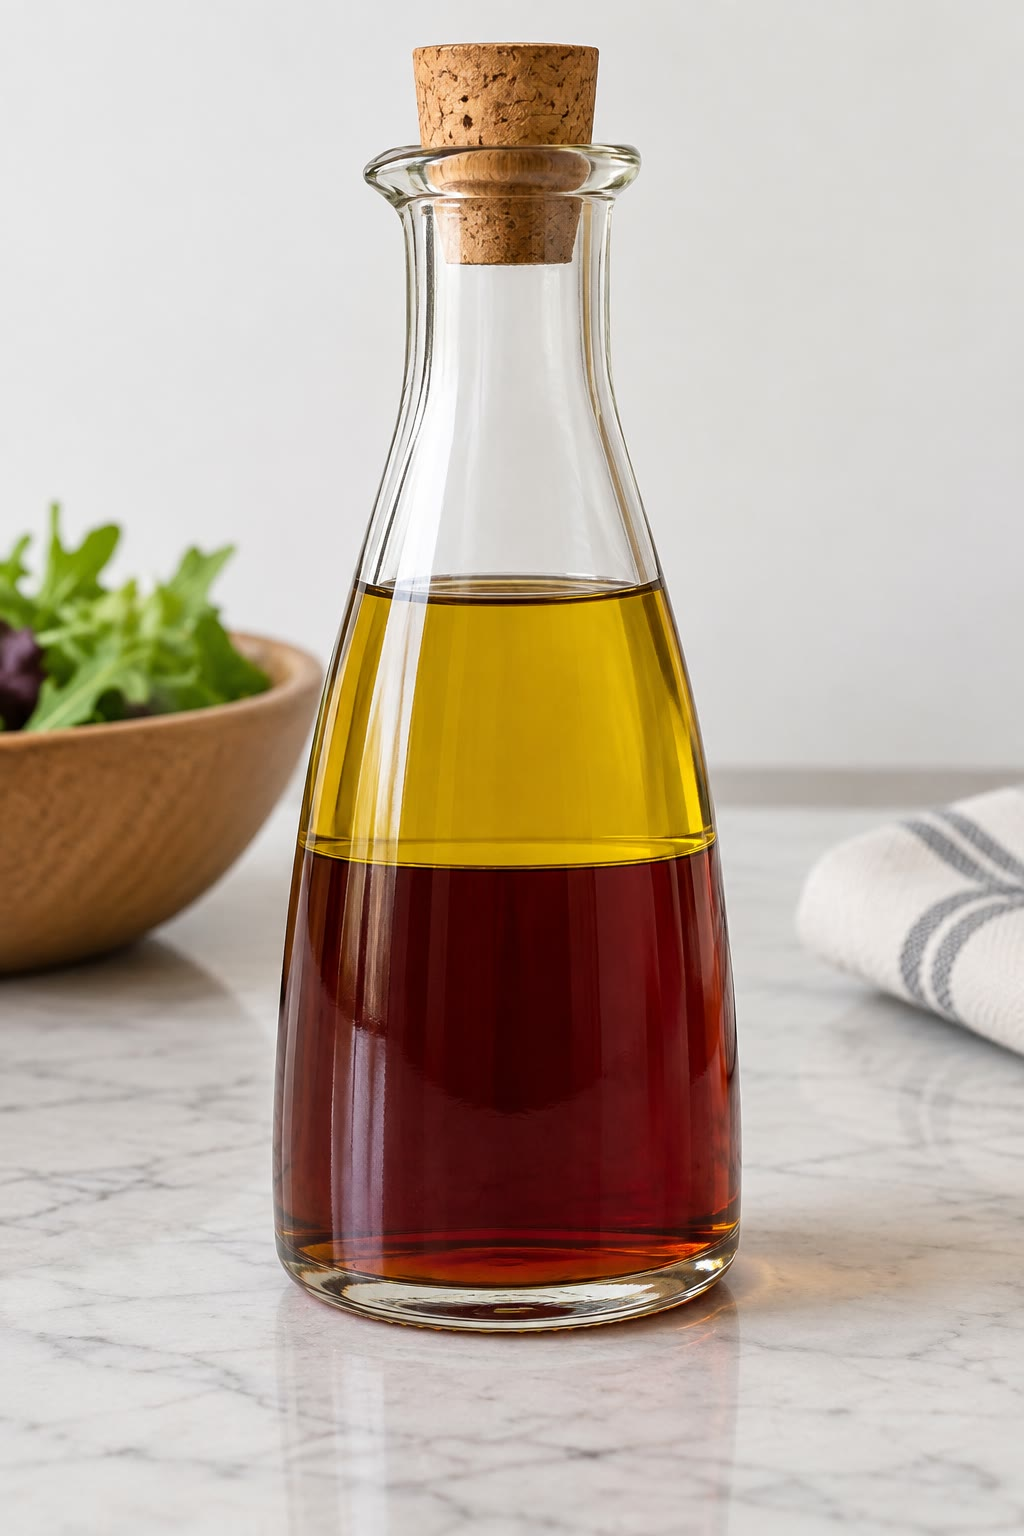
\includegraphics[width=0.2\linewidth]{images/book2/ai/b1-04-dressing.jpg}

{\small Um molho de salada em repouso: o azeite, apolar, flutua sobre o
vinagre, uma solução aquosa; os dois líquidos são imiscíveis.}
\end{omfigure}

\begin{definition}[Hidrofílico, hidrofóbico, anfifílico]\label{def:b1:intermolecular-forces-solvents:amphiphile}
Um grupo é \emph{hidrofílico}\index{hidrofilico@hidrofílico} quando interage
favoravelmente com a água (grupos iônicos ou polares: \ce{-COO^-}, \ce{-OH},
\ce{-SO3^-}) e \emph{hidrofóbico}\index{hidrofobico@hidrofóbico} quando não interage
(cadeias de hidrocarbonetos). Uma molécula é \emph{anfifílica}\index{anfifilico@anfifílico}
quando tem ao mesmo tempo uma cabeça hidrofílica e uma cauda hidrofóbica.
\end{definition}

\begin{example}[O sabão]\label{ex:b1:intermolecular-forces-solvents:soap}
O dodecanoato de sódio, \ce{CH3(CH2)10COO- Na+}, é \omterm{def:b1:intermolecular-forces-solvents:amphiphile}{anfifílico}. Na
superfície da água, suas moléculas ficam com a cabeça na água e a
cauda no ar. No interior do líquido, acima de uma pequena concentração,
elas se reúnem em esferas --- micelas --- com as caudas dentro e as
cabeças fora. A gordura, apolar, se dissolve no núcleo \omterm{def:b1:intermolecular-forces-solvents:amphiphile}{hidrofóbico} das
micelas e é levada embora pela água.
\end{example}

\begin{omfigure}
\begin{tikzpicture}[font=\small]
  % interface
  \fill[omWater] (-3.2,-1.6) rectangle (-0.4,0);
  \draw[omDef!60] (-3.2,0) -- (-0.4,0);
  \node[anchor=south west] at (-3.2,0.95) {ar};
  \node[anchor=north west] at (-3.2,-1.2) {água};
  \foreach \x in {-2.9,-2.5,...,-0.6} {
    \fill[omThm] (\x,-0.12) circle (0.11);
    \draw[thick, black!70, decorate, decoration={zigzag, amplitude=1pt, segment length=3pt}] (\x,0) -- (\x,0.85);
  }
  % micelle
  \begin{scope}[xshift=3.2cm, yshift=-0.4cm]
    \fill[omWater] (-2,-1.6) rectangle (2,1.6);
    \foreach \a in {0,30,...,330} {
      \draw[thick, black!70, decorate, decoration={zigzag, amplitude=1pt, segment length=3pt}] (\a:0.25) -- (\a:1.0);
      \fill[omThm] (\a:1.12) circle (0.11);
    }
    \node[anchor=north] at (0,-1.65) {uma micela na água};
  \end{scope}
\end{tikzpicture}

{\small Moléculas \omterm{def:b1:intermolecular-forces-solvents:amphiphile}{anfifílicas} (cabeça \omterm{def:b1:intermolecular-forces-solvents:amphiphile}{hidrofílica} vermelha, cauda
\omterm{def:b1:intermolecular-forces-solvents:amphiphile}{hidrofóbica} em zigue-zague) na superfície da água e reunidas em uma
micela, desenhada em corte; as micelas são estudadas no volume do 3.º ano.}
\end{omfigure}

\begin{method}[Escolher um solvente]\label{met:b1:intermolecular-forces-solvents:choose}
Para escolher um solvente para um soluto ou uma reação:
\begin{enumerate}
  \item caracterize o soluto: iônico, polar, capaz de doar ou aceitar
        \omterm{def:b1:intermolecular-forces-solvents:hbond}{ligações de hidrogênio}, ou apolar;
  \item escolha um solvente do mesmo tipo (\cref{prop:b1:intermolecular-forces-solvents:like}),
        com alta permissividade se for preciso separar íons;
  \item para uma reação entre um ânion e uma molécula, prefira um
        \omterm{def:b1:intermolecular-forces-solvents:solvent-classes}{solvente polar} aprótico, que dissolve o sal sem prender o ânion
        por \omterm{def:b1:intermolecular-forces-solvents:hbond}{ligações de hidrogênio} (\cref{ch:b1:nucleophilic-substitution});
  \item para uma extração, escolha um solvente imiscível com o primeiro
        e no qual o soluto seja muito mais solúvel.
\end{enumerate}
\end{method}

\section{Exercícios}

\begin{exercise}[$\star$]\label{exo:b1:intermolecular-forces-solvents:1}
Cite as interações presentes entre as partículas do argônio líquido, do
cloreto de hidrogênio líquido, da água líquida, do metano líquido e do
di-iodo sólido, e diga qual predomina em cada caso.
\end{exercise}

\begin{exercise}[$\star$]\label{exo:b1:intermolecular-forces-solvents:2}
Quais destas substâncias formam \omterm{def:b1:intermolecular-forces-solvents:hbond}{ligações de hidrogênio} entre suas
próprias moléculas: \ce{CH3OH}, \ce{CH3OCH3}, \ce{CH3NH2}, \ce{CH3F}, \ce{HF},
\ce{CH4}? Quais só podem aceitar \omterm{def:b1:intermolecular-forces-solvents:hbond}{ligações de hidrogênio} de outra molécula?
\end{exercise}

\begin{exercise}[$\star$]\label{exo:b1:intermolecular-forces-solvents:3}
Usando a tabela de solventes, classifique a água, o etanol, a propanona,
o hexano, o diclorometano e a acetonitrila como polares ou apolares,
próticos ou apróticos.
\end{exercise}

\begin{exercise}[$\star$]\label{exo:b1:intermolecular-forces-solvents:4}
Explique por que o di-iodo se dissolve muito melhor no hexano do que na
água, e por que o cloreto de sódio faz o contrário.
\end{exercise}

\begin{exercise}[$\star\star$]\label{exo:b1:intermolecular-forces-solvents:5}
O metanol ferve a \qty{64.7}{\celsius}, o etanol a \qty{78.4}{\celsius},
o ácido etanoico a \qty{118.1}{\celsius} e o metoximetano a
\qty{-25.0}{\celsius}. Explique essa ordem.
% ledger: bp:CH3OH, bp:C2H5OH, bp:CH3COOH, bp:CH3OCH3
\end{exercise}

\begin{exercise}[$\star\star$]\label{exo:b1:intermolecular-forces-solvents:6}
Calcule a força de Coulomb entre um íon \ce{Na+} e um íon \ce{Cl-}
separados por \qty{500}{pm} no vácuo ($\varepsilon_0 = \qty{8.854e-12}{F/m}$,
$e = \qty{1.602e-19}{C}$), depois na água ($\varepsilon_r = 78.4$) e no
hexano ($\varepsilon_r = 1.89$). Comente.
\end{exercise}

\begin{exercise}[$\star\star$]\label{exo:b1:intermolecular-forces-solvents:7}
A propanona e a água são \omterm{def:b1:intermolecular-forces-solvents:miscibility}{miscíveis} em quaisquer proporções; o hexano e a
água não. Explique, considerando as interações rompidas e formadas.
\end{exercise}

\begin{exercise}[$\star\star$]\label{exo:b1:intermolecular-forces-solvents:8}
\ce{HCl} tem \omterm{def:b1:lewis-resonance-vsepr:dipole}{momento dipolar} de \qty{1.09}{\debye} e ferve a
\qty{-85.0}{\celsius}; \ce{HBr} tem \qty{0.83}{\debye} e ferve a
\qty{-66.4}{\celsius}. Por que a molécula menos polar ferve a uma
temperatura mais alta?
% ledger: dip:HCl, dip:HBr, bp:HCl, bp:HBr
\end{exercise}

\begin{exercise}[$\star\star$]\label{exo:b1:intermolecular-forces-solvents:9}
Desenhe o dímero cíclico do ácido etanoico. Em solução no benzeno, o
ácido etanoico se comporta como se sua massa molar fosse cerca do dobro
de \qty{60}{g/mol}; na água, não. Explique os dois fatos.
\end{exercise}

\begin{exercise}[$\star\star\star$]\label{exo:b1:intermolecular-forces-solvents:10}
Descreva a dissolução do cloreto de sódio na água em termos de
dissociação e \omterm{def:b1:intermolecular-forces-solvents:dissolution}{solvatação}, e a do cloreto de hidrogênio na água em termos
de ionização, dissociação e \omterm{def:b1:intermolecular-forces-solvents:dissolution}{solvatação}. Por que o cloreto de hidrogênio
no hexano dá uma solução que não conduz?
\end{exercise}

\begin{exercise}[$\star\star\star$]\label{exo:b1:intermolecular-forces-solvents:11}
A partir das temperaturas de ebulição dos alcanos lineares (pentano
\qty{36.1}{\celsius}, decano \qty{174.1}{\celsius}), calcule o aumento
médio por grupo \ce{CH2} entre \ce{C5} e \ce{C10} e estime a temperatura
de ebulição do undecano. Por que o incremento diminui ao longo da
série?
% ledger: bp:C5H12, bp:C10H22
\end{exercise}

\begin{exercise}[$\star\star\star$]\label{exo:b1:intermolecular-forces-solvents:12}
O dodecilsulfato de sódio, \ce{CH3(CH2)11OSO3^- Na+}, é um detergente.
Identifique suas partes \omterm{def:b1:intermolecular-forces-solvents:amphiphile}{hidrofílica} e \omterm{def:b1:intermolecular-forces-solvents:amphiphile}{hidrofóbica}, esboce seu arranjo na
superfície da água e em uma micela, e explique como ele remove uma
mancha de gordura de um tecido.
\end{exercise}

\section{Problema: Se a água não tivesse ligações de hidrogênio}

\begin{problem}[{Problema de fim de semana --- as forças de London nos
gases nobres e nos alcanos, a escolha de um solvente e a temperatura de
ebulição que a água teria sem ligações de hidrogênio}]
\label{pb:b1:intermolecular-forces-solvents:1}
Temperaturas de ebulição sob \qty{1}{atm} (em \unit{\celsius}): \ce{He} $-268.9$,
\ce{Ne} $-246.1$, \ce{Ar} $-185.9$, \ce{Kr} $-153.4$, \ce{Xe} $-108.1$;
pentano 36.1, hexano 68.8; \ce{CH4} $-161.5$, \ce{SiH4} $-112.0$,
\ce{GeH4} $-88.1$; \ce{NH3} $-33.4$, \ce{PH3} $-87.8$, \ce{AsH3} $-62.5$;
\ce{H2O} 100.0, \ce{H2S} $-60.3$, \ce{H2Se} $-41.3$; \ce{HF} 19.6,
\ce{HCl} $-85.0$, \ce{HBr} $-66.4$.
% ledger: bp:He, bp:Ne, bp:Ar, bp:Kr, bp:Xe, bp:C5H12, bp:C6H14, bp:CH4,
% bp:SiH4, bp:GeH4, bp:NH3, bp:PH3, bp:AsH3, bp:H2O, bp:H2S, bp:H2Se,
% bp:HF, bp:HCl, bp:HBr

\medskip
\noindent\textbf{Parte I --- Só London.}
\begin{enumerate}
  \item Que interação mantém unidos os átomos do argônio líquido?
  \item Explique o aumento da temperatura de ebulição do hélio ao xenônio.
  \item Por que a temperatura de ebulição do hélio é a mais baixa de
        todas as substâncias?
  \item Compare o pentano e o hexano: o que acrescenta um grupo \ce{CH2}?
  \item Metano, silano e germano não têm \omterm{def:b1:lewis-resonance-vsepr:dipole}{momento dipolar}. Que
        interação explica a ordem de suas temperaturas de ebulição?
  \item Por que nenhuma \omterm{def:b1:intermolecular-forces-solvents:hbond}{ligação de hidrogênio} é possível no metano?
\end{enumerate}

\medskip
\noindent\textbf{Parte II --- A escolha dos solventes.}
Use a tabela de solventes do capítulo.
\begin{enumerate}[resume]
  \item Qual solvente da tabela dissolve melhor o cloreto de sódio, e
        por quê?
  \item Por qual fator a atração entre dois íons é menor na água do que
        no hexano, à mesma distância?
  \item Uma reação entre o ânion \ce{CN-} e uma molécula orgânica deve
        ser feita em um solvente que dissolva o sal, mas não prenda o
        ânion por \omterm{def:b1:intermolecular-forces-solvents:hbond}{ligações de hidrogênio}. Escolha um.
  \item Para extrair o di-iodo de uma solução aquosa, que solvente da
        tabela você escolheria, e em que fase o iodo vai acabar?
  \item Explique por que o etanol não pode ser usado nessa extração.
  \item O etoxietano é pouco \omterm{def:b1:intermolecular-forces-solvents:miscibility}{miscível} com a água, embora seja polar.
        Proponha uma explicação.
\end{enumerate}

\medskip
\noindent\textbf{Parte III --- Os outros hidretos.}
\begin{enumerate}[resume]
  \item Para o \omterm{def:b1:periodicity:table}{grupo} 17, calcule a variação da temperatura de ebulição de
        \ce{HCl} para \ce{HBr} e extrapole a mesma variação de volta ao
        \omterm{def:b1:periodicity:table}{período} 2.
  \item Compare o valor extrapolado com a temperatura de ebulição de \ce{HF}.
  \item Mesmas duas perguntas para o \omterm{def:b1:periodicity:table}{grupo} 15 (\ce{PH3}, \ce{AsH3} e
        \ce{NH3}).
  \item Para o \omterm{def:b1:periodicity:table}{grupo} 14, \ce{CH4} fica acima ou abaixo da extrapolação a
        partir de \ce{SiH4} e \ce{GeH4}? Por que isso não surpreende?
  \item Ordene os excessos de \ce{NH3}, \ce{HF} e da água.
  \item Conte as \omterm{def:b1:intermolecular-forces-solvents:hbond}{ligações de hidrogênio} que cada molécula de \ce{NH3},
        \ce{HF} e \ce{H2O} pode doar e aceitar, e explique essa ordem.
\end{enumerate}

\medskip
\noindent\textbf{Parte IV --- A água sem \omterm{def:b1:intermolecular-forces-solvents:hbond}{ligações de hidrogênio}.}
\begin{enumerate}[resume]
  \item Por que \ce{H2S} e \ce{H2Se} servem para uma extrapolação, e por
        que não a própria água?
  \item Calcule a variação da temperatura de ebulição de \ce{H2S} para
        \ce{H2Se}.
  \item Escreva a equação da reta que passa por esses dois pontos, com o
        \omterm{def:b1:periodicity:table}{período} $p$ como variável.
  \item Deduza a temperatura de ebulição que a água teria em $p = 2$.
  \item Em quanto as \omterm{def:b1:intermolecular-forces-solvents:hbond}{ligações de hidrogênio} elevam a temperatura de
        ebulição da água?
  \item Conclua: a que temperatura a água ferveria se suas moléculas se
        atraíssem como as de \ce{H2S}?
\end{enumerate}
\end{problem}
